%!TEX encoding = UTF-8 Unicode  
\chapter{表格、图片和公式}
\section{数学公式}
这一部分列举了一些常用公式和数学符号的在中的表示方法。

常用数学符号:

$\{(\mathbf{x_i},l_i),i=1,2,...,n\}$

$\mathbf{x_i}\in \Re ^d$

$\mathbf{c}=[c_1,c_2,...,c_n]^T$

$\left \lVert c \right \rVert_0$

$\left \lVert \mathbf{v} \right \rVert_p = (\sum_i |v_i|^p)^{1/p}$

$\int_{0}^{\infty}f(t\mid\alpha,\beta)dt$

\vskip 20pt

最一般的公式:
\begin{equation}
\label{eq:orginal}
\mathbf{y}=c_1\mathbf{x_1}+c_2\mathbf{x_2}+...+c_n\mathbf{x_n}
\end{equation}

\begin{equation}
\label{eq:spareserep}
c=\mathop{\mathrm{min}}\limits_{c'\in\Re^n} \left \lVert c' \right \rVert_0, \quad \text{subject to} \quad \mathbf{y}=Ac
\end{equation}

\vskip 20pt

需要分两行或多行显示的公式:
\begin{equation}
\begin{array}{l}
g(\mathbf{x})=-8.2+0.031\text{Age}+0.013\text{HR}-0.35\text{Albumin}+0.042\text{ALP}\\
\quad \quad \quad -0.015\text{AST}+0.389\text{Ratio}-0.009\text{PaO2}+0.395\text{FiO2}\\
\end{array}
\end{equation}

\vskip 20pt

多个方程,使用同一个编号:
\begin{equation}\label{eq:definefeature}
   \begin{array}{l}
\text{if \quad}  \bar{v} \le v_2 \text{\quad and \quad} \underline{v} \ge v_1, \text{\quad then \quad} v=0;\\
\text{else \quad} v=\text{max}\{\bar{v}-v_2,v_1-\underline{v}\}
\end{array}
\end{equation}

带大括号的方程:
\begin{equation}
\left\{
\begin{aligned}
    \frac{\partial(\log L(\alpha,\beta))}{\partial \alpha}&=0  \\
    \frac{\partial(\log L(\alpha,\beta))}{\partial \beta}&=0   \\
\end{aligned}
\right.
\end{equation}

矩阵形式的方程:
\begin{displaymath}
E[(\hat{\tilde{x}}-E[\hat{\tilde{x}}])  {(\hat{\tilde{x}}-E[\hat{\tilde{x}}])}^T]=
\begin{bmatrix}
\mathbf{P}_{{x_k}{x_k}}  & \mathbf{P}_{{x_k}{w_k}}\\
\mathbf{P}_{{w_k}{x_k}} &  \mathbf{P}_{{w_k}{w_k}}
\end{bmatrix}
\end{displaymath}

\section{表格}
普通的表格(\ref{tab:modelprocess}和\ref{tab:normal}):
\begin{table}
\begin{center}
\begin{tabular}{@{}cc@{}} \toprule
序号 \quad \quad & 内容\\
\midrule	
1	&准确定义评估系统关注的结果\\
\midrule
2	&定义可能的预测变量\\
\midrule
3	&数据收集\\
\midrule
4	&单变量分析($\chi ^2$检验,学生$t$检验)\\
\midrule
\bottomrule
\end{tabular}
\end{center}
\caption{普通的表格A}
\label{tab:modelprocess}
\end{table}

\begin{table}[htbp]
\begin{center}
\begin{tabular}{cc| cc} \toprule
生理量(单位) \quad  & 参考值 &生理量(单位) \quad & 参考值\\
\hline
HR(bpm) & $70 \sim 109$ & SysABP(mmHg) & $80 \sim 149$ \\
\hline
Temp(\textcelsius) & $36 \sim 38.4$ & BUN(mg/mL) & $9.8 \sim 20.7$\\
\hline
RespRate(bpm)& $12 \sim 24$ & PaO2/FiO2(mmHg)& $>300$ \\
\bottomrule
\end{tabular}
\end{center}
\caption{普通的表格B}
\label{tab:normal}
\end{table}

可以用作流程图的表格(\ref{tab:SpareseRep}):
\begin{table}
\begin{center}
\begin{tabular}{@{}ccc@{}} \toprule
\bf{Inputs:} \quad  & $ \{(\mathbf{x_i},l_i);i=1,...,n \} $ and $\mathbf{y} $ \\
1 & $\mathbf{x_i}$和$\mathbf{y}$的归一化  \\
2 & 构造矩阵$A$  \\
3 & 解优化问题\\
4 &	计算 $g_k(\mathbf{y}),k=0,1$	\\
\bf{Output:} \quad & arg $\mathop{\mathrm{min}}\limits_{k} g_k(\mathbf{y}) $\\
\bottomrule
\end{tabular}
\end{center}
\caption{可以用作流程图的表格}
\label{tab:SpareseRep}
\end{table}

同时跨行跨列的表格(\ref{tab:confusionmatrix}):
\begin{table}[htbp]
\centering
\begin{tabular}{rcccc}
    \toprule
    \multicolumn{2}{c}{\multirow{2}[2]{*}{Outcome}} & \multicolumn{2}{c}{Observed} & \\
    \multicolumn{2}{c}{} & Death  & Survivor \\
    \cline{3-5}
    \multirow{2}[4]{*}{Predicted} & Death & TP   & FP \\
    \cline{3-5}
          & Survivor & FN   & TN \\
   \bottomrule
\end{tabular}
\caption{同时跨行跨列的表格}
\label{tab:confusionmatrix}
\end{table}


\section{图片}
单幅图片(\ref{fig:histogram})和多幅图片(\ref{fig:ROC})
\begin{figure}[htbp]
\begin{center}
	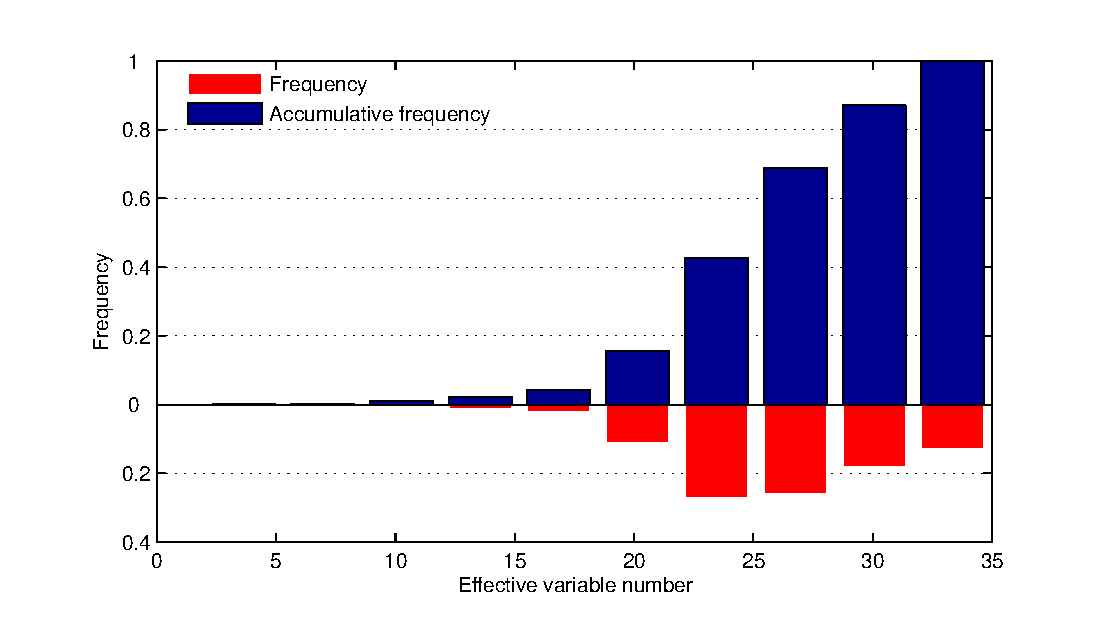
\includegraphics[width=0.8\linewidth]{histogram.eps}
\end{center}
\caption{单幅图片}
\label{fig:histogram}
\end{figure}

\begin{figure}
\begin{center}
\subfloat[年龄的ROC曲线]{
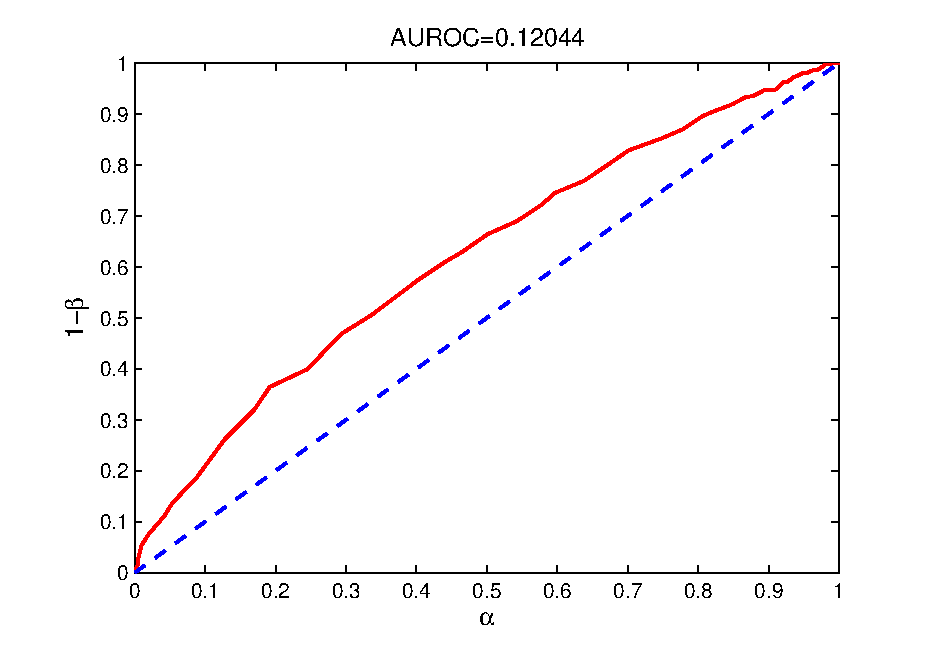
\includegraphics[width=0.5\textwidth]{Fig_A.eps}}
\subfloat[体重的ROC曲线]{
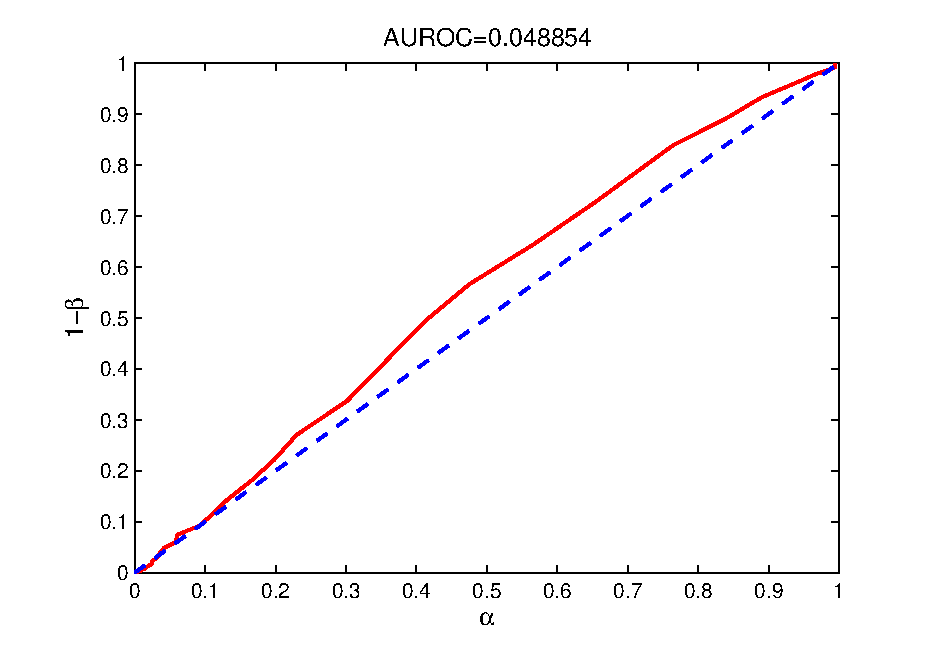
\includegraphics[width=0.5\linewidth]{Fig_B.eps}}\\
\subfloat[年龄频率分布直方图]{
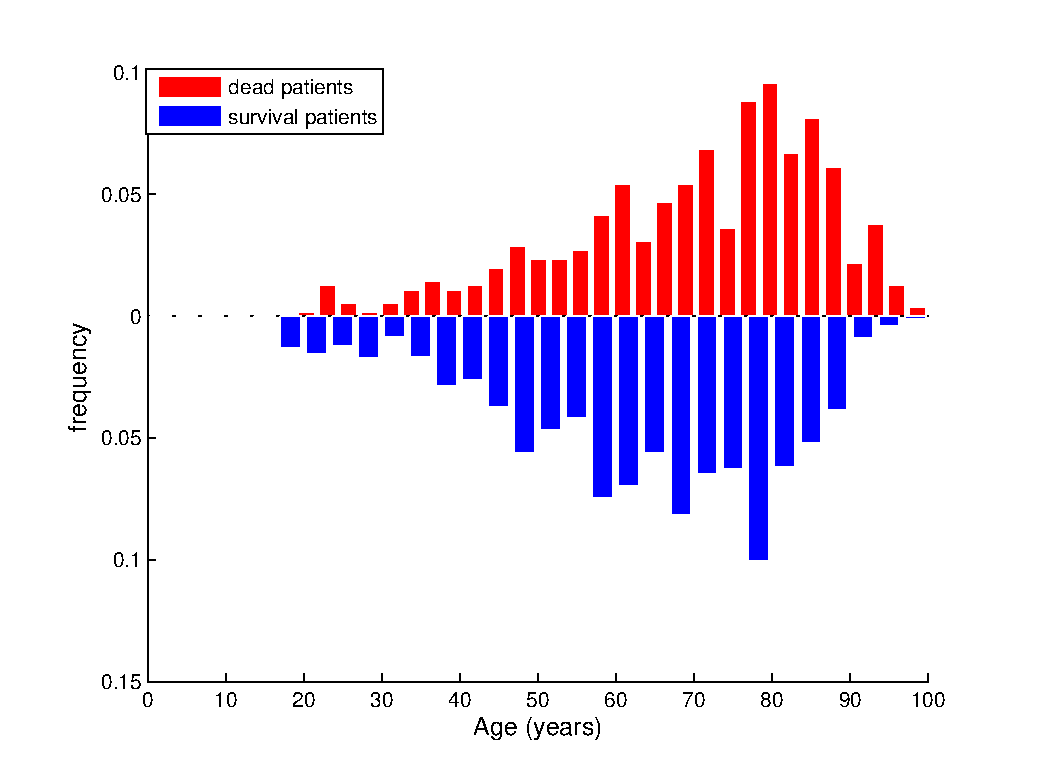
\includegraphics[width=0.5\textwidth]{Fig_C.eps}}
\subfloat[体重频率分布直方图]{
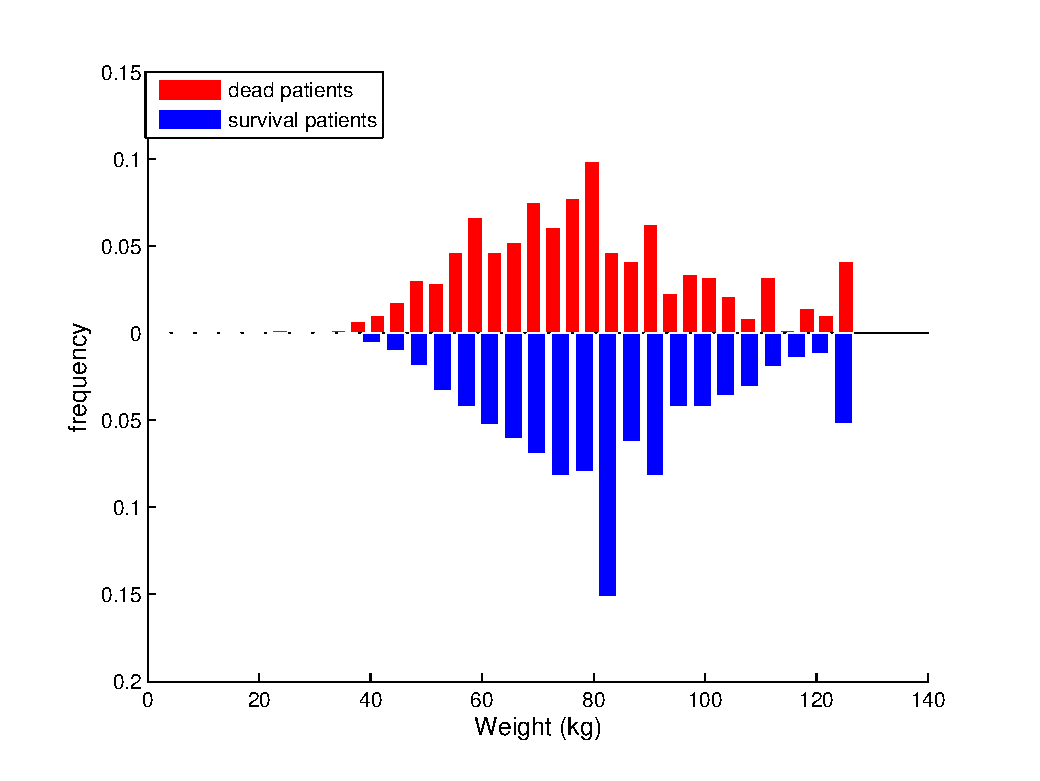
\includegraphics[width=0.5\linewidth]{Fig_D.eps}}
\end{center}
\caption{多幅图片}
\label{fig:ROC}
\end{figure}

\chapter{关于参考文献}
所有参考文献的条目都在文件refs.bib中。新建参考文献的最简单方法,就是利用Google Scholar提供的“导入BibTeX”功能。

\begin{figure}[htbp]
\begin{center}
	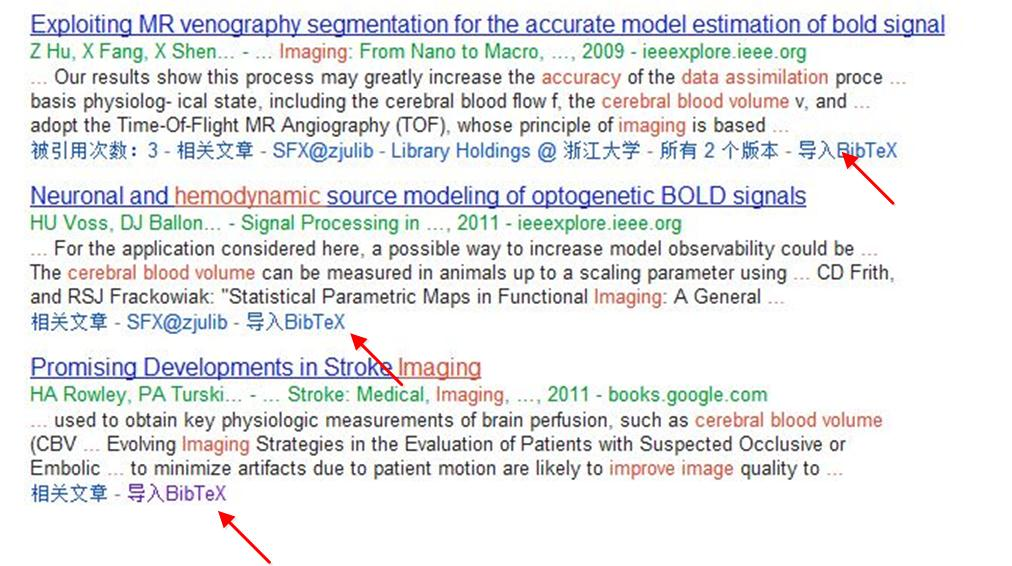
\includegraphics[width=0.8\linewidth]{google.jpg}
\end{center}
\caption{Google Scholar的导入BibTeX功能}
\label{fig:google}
\end{figure}

\cite{knaus1981apache}、\cite{website:challenge}、\cite{hug2009icu}和\cite{jobson2005applied}分别给出了期刊论文、网址、会议合集论文以及书籍的
参考文献引用格式。

\chapter{写在最后}
由于模板使用了书籍排版的基本样式,所以在一个章节末尾的双数页可能会是空白页,这适合于双面打印。如果你想去掉空白页,简单的办法是直接在Adobe Acrobat中删除页面。而如果您想大修此模板,请阅读和修改文件ZJUthesis.cls和ZJUthesis.cfg。

作为一名不到一个月就要毕业的光电大四同学,这份模板就算是临走前送给学弟学妹的一个礼物吧。由于本人也是菜鸟,水平有限,所以模板中还有一些
Bug不能更正,而且格式上和系里提供的WORD模板还有些出入。在这里抛砖引玉,
只是希望更多真正懂的同学能把它完善,从而使大家受益{\LARGE{\Smiley}}。 